
\labday{Thread Pool}

\experiment{Threads}
A {\bf Thread} is a logical flow that runs in the context of the program.  Threads share all the same date structures (virtual address space), processes DO NOT.  It is also important to note that each thread has its own thread context including a unique integer thread ID (TID), stack,stack pointer, program counter, general purpose registers, and condition codes.\\

Threads  are scheduled automatically by the kernel and are known by an integer ID.\\
Each process begins life as a single thread called the main thread.  At some point the main thread creates a peer thread, and from this point in time the two threads run concurrently.  Eventually, control passes to the peer thread via a context switch, because the main thread is doing something slow (read, sleep, or disk access).\\

Threads are organized in a pool of peers.  The main thread is different in that it is always the first thread to run in the process.  Each peer can read and write the same shared data.\\

Variables in threaded C programs are mapped to virtual memory according to their storage classes:
\begin{itemize}
\item Global Variables (Shared):  A global variable is any variable declared outside of a function.  At run, the read/write area of virtual memory contains exactly one instance of each global variable that can be referenced by any thread.
\item Local Automatic Variables (Not Shared): This is a variable declared inside a function WITHOUT the static attribute.  At run time, each thread's stack contains its own instances of any local automatic variables.
\item Local Static Variables (Shared):  This is a variable declared inside a function with the static attribute.  As with global variables , the read/write area of virtual memory contains exactly one instance of each local static variable in our program.
\end{itemize}


\begin{lstlisting}
#include <stdio.h>
#include <pthread.h>

#define NUMTHRDS 2

pthread_t t [ NUMTHRDS];
int coin_flip;

pthread_mutex_t flip_done;
static void *thread2(void *_){
	pthread_mutex_lock(&flip_done);
	printf("Thread 2: flipped coin %d\n", coin_flip);
}


static void * thread1(void * _)
{
	coin_flip = 1;
	pthread_mutex_unlock(&flip_done);
	printf("Thread 1: flipped coin %d\n", coin_flip);
}
int main()
{
	pthread_mutex_init(&flip_done, NULL);
	pthread_mutex_lock(&flip_done);
	pthread_create(&t[1], NULL, thread2, NULL);
	pthread_create(&t[0], NULL, thread1, NULL);
	 pthread_mutex_destroy(&flip_done);
	//must have this as main will block until all the supported threads are done
	pthread_exit(NULL);
	return 1;
}


\end{lstlisting}


\experiment{Race Conditions}
One thing to watch out for in threads is a race condition.  A race condition occurs when two or more threads read and write a shared variable, and the final result depends on the execution of those threads.


\experiment{Deadlock and Livelock}
Deadlocks can occur when two or more threads are each waiting for the other to finish, and thus neither gets done.  The picture below illustrates this point.  Imagine that one thread executes the code on the left (we will that thread X) and another thread executes the code on the right (Thread Y).  Now thread X executes and grabs the mutex A, while thread Y executes and grabs mutex B.  Thread X understands that it must wait for  mutex B to become available.  However thread Y is also waiting to obtain mutex A.  Both threads are waiting for another thread to give something up that it will not and we have a deadlock.



\begin{center}
    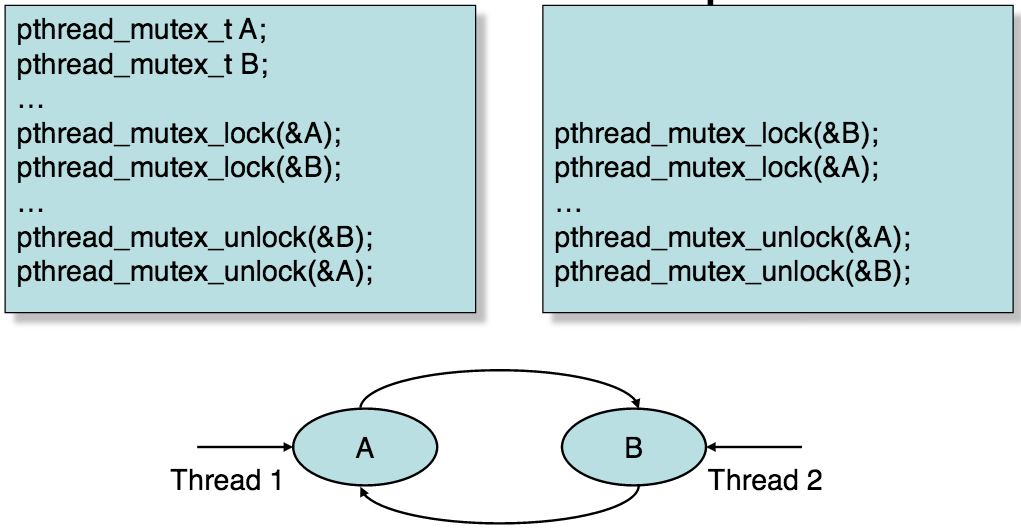
\includegraphics[scale=0.5]{threads/deadlock.png}
\end{center}

\experiment{Semaphores}
A semaphore is a variable or abstract data type that is used for controlling access to multiple threads or processes

Semaphores provide a great way to ensure mutuaally exclusive access to shared variables.  A semaphore that is used to protect shared variables is called a binary semaphore becuase its value is always 0 or 1.\\

Another important use of semaphores ,besides providing mutual exclusion, is to schedule accesses to shared rescources.\\

Think of semaphores as bouncers at a nightclub. There are a dedicated number of people that are allowed in the club at once. If the club is full no one is allowed to enter, but as soon as one person leaves another person might enter.
